% This is "sig-alternate.tex" V2.1 April 2013
% This file should be compiled with V2.5 of "sig-alternate.cls" May 2012
%
% This example file demonstrates the use of the 'sig-alternate.cls'
% V2.5 LaTeX2e document class file. It is for those submitting
% articles to ACM Conference Proceedings WHO DO NOT WISH TO
% STRICTLY ADHERE TO THE SIGS (PUBS-BOARD-ENDORSED) STYLE.
% The 'sig-alternate.cls' file will produce a similar-looking,
% albeit, 'tighter' paper resulting in, invariably, fewer pages.
%
% ----------------------------------------------------------------------------------------------------------------
% This .tex file (and associated .cls V2.5) produces:
%       1) The Permission Statement
%       2) The Conference (location) Info information
%       3) The Copyright Line with ACM data
%       4) NO page numbers
%
% as against the acm_proc_article-sp.cls file which
% DOES NOT produce 1) thru' 3) above.
%
% Using 'sig-alternate.cls' you have control, however, from within
% the source .tex file, over both the CopyrightYear
% (defaulted to 200X) and the ACM Copyright Data
% (defaulted to X-XXXXX-XX-X/XX/XX).
% e.g.
% \CopyrightYear{2007} will cause 2007 to appear in the copyright line.
% \crdata{0-12345-67-8/90/12} will cause 0-12345-67-8/90/12 to appear in the copyright line.
%
% ---------------------------------------------------------------------------------------------------------------
% This .tex source is an example which *does* use
% the .bib file (from which the .bbl file % is produced).
% REMEMBER HOWEVER: After having produced the .bbl file,
% and prior to final submission, you *NEED* to 'insert'
% your .bbl file into your source .tex file so as to provide
% ONE 'self-contained' source file.
%
% ================= IF YOU HAVE QUESTIONS =======================
% Questions regarding the SIGS styles, SIGS policies and
% procedures, Conferences etc. should be sent to
% Adrienne Griscti (griscti@acm.org)
%
% Technical questions _only_ to
% Gerald Murray (murray@hq.acm.org)
% ===============================================================
%
% For tracking purposes - this is V2.0 - May 2012



\documentclass{sig-alternate-05-2015}

\begin{document}

% Copyright
\setcopyright{acmcopyright}
%\setcopyright{acmlicensed}
%\setcopyright{rightsretained}
%\setcopyright{usgov}
%\setcopyright{usgovmixed}
%\setcopyright{cagov}
%\setcopyright{cagovmixed}


% DOI
\doi{10.475/123_4}

% ISBN
\isbn{123-4567-24-567/08/06}

%Conference
\conferenceinfo{PLDI '13}{June 16--19, 2013, Seattle, WA, USA}

\acmPrice{\$15.00}

%
% --- Author Metadata here ---
\conferenceinfo{WOODSTOCK}{'97 El Paso, Texas USA}
%\CopyrightYear{2007} % Allows default copyright year (20XX) to be over-ridden - IF NEED BE.
%\crdata{0-12345-67-8/90/01}  % Allows default copyright data (0-89791-88-6/97/05) to be over-ridden - IF NEED BE.
% --- End of Author Metadata ---

\title{ Mining HIV Trends in Social Media Data}
%
% You need the command \numberofauthors to handle the 'placement
% and alignment' of the authors beneath the title.
%
% For aesthetic reasons, we recommend 'three authors at a time'
% i.e. three 'name/affiliation blocks' be placed beneath the title.
%
% NOTE: You are NOT restricted in how many 'rows' of
% "name/affiliations" may appear. We just ask that you restrict
% the number of 'columns' to three.
%
% Because of the available 'opening page real-estate'
% we ask you to refrain from putting more than six authors
% (two rows with three columns) beneath the article title.
% More than six makes the first-page appear very cluttered indeed.
%
% Use the \alignauthor commands to handle the names
% and affiliations for an 'aesthetic maximum' of six authors.
% Add names, affiliations, addresses for
% the seventh etc. author(s) as the argument for the
% \additionalauthors command.
% These 'additional authors' will be output/set for you
% without further effort on your part as the last section in
% the body of your article BEFORE References or any Appendices.

\numberofauthors{2} %  in this sample file, there are a *total*
% of EIGHT authors. SIX appear on the 'first-page' (for formatting
% reasons) and the remaining two appear in the \additionalauthors section.
%
\author{
% You can go ahead and credit any number of authors here,
% e.g. one 'row of three' or two rows (consisting of one row of three
% and a second row of one, two or three).
%
% The command \alignauthor (no curly braces needed) should
% precede each author name, affiliation/snail-mail address and
% e-mail address. Additionally, tag each line of
% affiliation/address with \affaddr, and tag the
% e-mail address with \email.
%
% 1st. author
\alignauthor
Patrick Breen\\
       \affaddr{The Institute of Bioinformatics}\\
       \affaddr{The University of Georgia}\\
       \affaddr{Athens, Georgia}\\
       \email{pbreen@uga.edu}
% 2nd. author
\alignauthor
Shannon Quinn\titlenote{Corresponding author.}\\
       \affaddr{Institute of Computer Science}\\
       \affaddr{University of Georgia}\\
       \affaddr{Athens, Georgia}\\
       \email{squinn@cs.uga.edu}
}



\maketitle
\begin{abstract}

Here is the abstract.

\end{abstract}


%
% The code below should be generated by the tool at
% http://dl.acm.org/ccs.cfm
% Please copy and paste the code instead of the example below. 
%
% TODO: this section
\begin{CCSXML}

\end{CCSXML}


%
% End generated code
%

%
%  Use this command to print the description
%
\printccsdesc

% We no longer use \terms command
%\terms{Theory}

\keywords{ Social Media, Topic Modelling, Document Embedding}

\section{Introduction}

Introduce and literature review of:
1) PrEP, HIV, Twitter


2) Word2Vec, Doc2Vec


3) Dynamic Topic models, Latent Dirichlet allocation


\section{Results}

1.2 Million tweets related to 'hiv', 'aids', 'truvada', 'prophylaxis', 'imtesting', 'sexwork', 'gay', 'PrEP', were collected from Twitter's streaming API. The tweets were restricted to English language, and the collection dates spanned from the 47th week of 2015 to the 7th week of 2016. The tweets were lowercased, and cleaned of exotic characters.

Then a variety of analyses were run, each with their own additional preprocessing. These analyses sought to determine what things Twitter users were saying about HIV and PrEP, ultimately to determine how to coordinate public health efforts to promote PrEP adoption and adherence for at-risk individuals.

While we excluded non-English tweets, we found that the subset of tweets that had geolocation data available came from around the world. Tweets were concentrated on English speaking areas with high population (Figure 1).

\begin{figure}
\centering
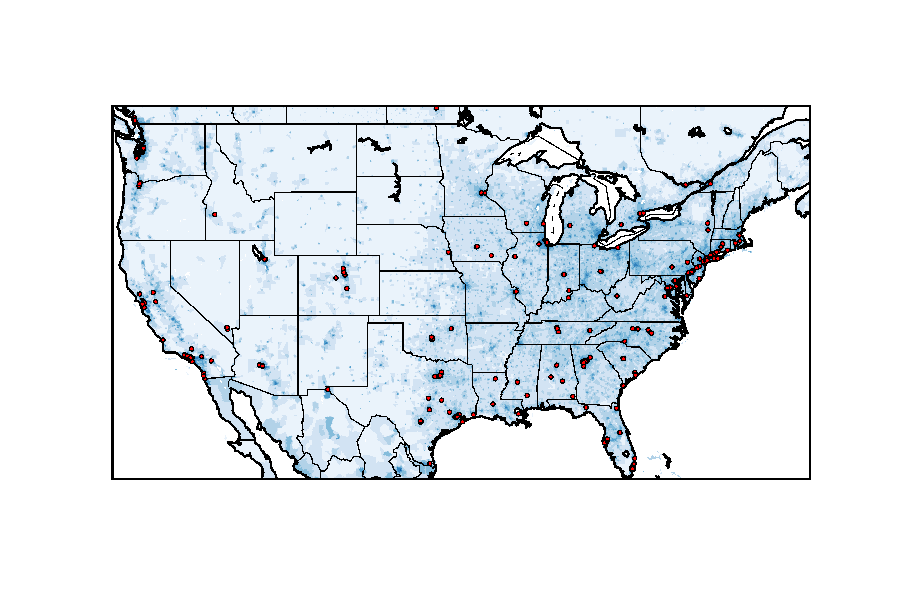
\includegraphics[height=2.5in, width=3.5in]{map}
\caption{Plot of geolocated tweets.}
\end{figure}

\subsection{Word and Document Similarity}

The first analyses that we performed sought to identify certain keywords, and hashtags that users were users were mentioning in PrEP related contexts. Word2Vec and the refinement, Paragraph2Vec are unsupervised machine learning methods that have performed well at embedding natural language in a semantic vector space.

We queried for the top 10 words that had the highest semantic similarity with the word 'truvada' (Table 1). We found many HIV related words, with the specific word 'prep' as the most similar.

Next we preformed Paragraph clustering. In this application, a paragraph is equivalent to the text of a tweet. In this method, we identify the similarity between tweets, and tweet-level attributes such as hashtags. Querying for the Paragraph-Vectors with high similarity to '\#truvada' identifies '\#prep' as the top related hashtag (Table 2). Furthermore, we see hashtags related to prevention, and HIV in the results.

The numeric entries in Table 2 correspond to tweet ID numbers. The top tweet associated with '\#truvada' has text: "\#girlsbelike if you see this 13 symptoms. do hiv test immediately. please read". This tweet is an HIV symptom related news update, which is representative of a large number of HIV related tweets on Twitter.

The combined results from Word2Vec and Paragraph2Vec demonstrate that we can scan through the Twitter corpus and find words, hashtags, and tweets that are semantically related to our PrEP query terms. When HIV public health researchers identify an important keyword, or hashtag, they can quickly use this method to identify related keywords and specific relevant tweets.

% table 1
\begin{table}
\centering
\caption{Cosine Similarity to 'truvada'}
\begin{tabular}{|l|c|} \hline
Related Word & Cosine Similarity to 'truvada'\\ \hline
prep & 0.836507\\ \hline
charliesheen & 0.774535\\ \hline
worldaidsday & 0.759242\\ \hline
hivtestweek & 0.797361\\ \hline
hiv & 0.744817\\ \hline
hivaids & 0.730966\\ \hline
aidsfreefuture & 0.721897\\ \hline
icasa2015 & 0.713624\\ \hline
benegative & 0.709129\\ \hline
martinshkreli & 0.702565\\ \hline
\hline\end{tabular}
\end{table}

% table 2
\begin{table}
\centering
\caption{Cosine Similarity to '\#truvada'}
\begin{tabular}{|l|c|} \hline
Related Hashtag/Tweet & Cosine Similarity to '\#truvada'\\ \hline
\#prep & 0.740855\\ \hline
\#hiv & 0.646245\\ \hline
685501883448963072 & 0.582529\\ \hline
\#prevention & 0.0.578786\\ \hline
\#potus & 0.561461\\ \hline
688733331081527296 & 0.558048\\ \hline
\#[Japanese "email friend"] & 0.557464\\ \hline
\#[Japanese "sex friend"] & 0.556990\\ \hline
\#bbbh & 0.547450\\ \hline
\#cure & 	0.545497\\ \hline
\hline\end{tabular}
\end{table}


\subsection{Time Domain}

Next we sought to identify some temporal trends in PrEP related trends. We used Dynamic Topic Modelling to identify how certain topics change over time. We specified 10 topics and plotted representative words from two of the topics.

In topic 3 we see that the keyword 'prep' remains relatively constant, while 'prevention' and 'truvada' decline over time. 'hivaids' increases and then decreases in magnitude over the course of the time series (Figure 2). These dynamics may indicate short term events in hivaids and PrEP-related conversation on twitter over the time period studied.

We found that topic 5 captured several keywords related to World AIDS Day (Figure 3). We can see that all of these terms peak in the 47th week of 2015 and then decline into 2016. This correlates well with the actual date of World AIDS Day, December 1st. While we aren't specifically interested in World AIDS Day to inform our understanding of PrEP discussion, this observation validates our ability to identify temporal events using DTM.

% figure 2
\begin{figure}
\centering
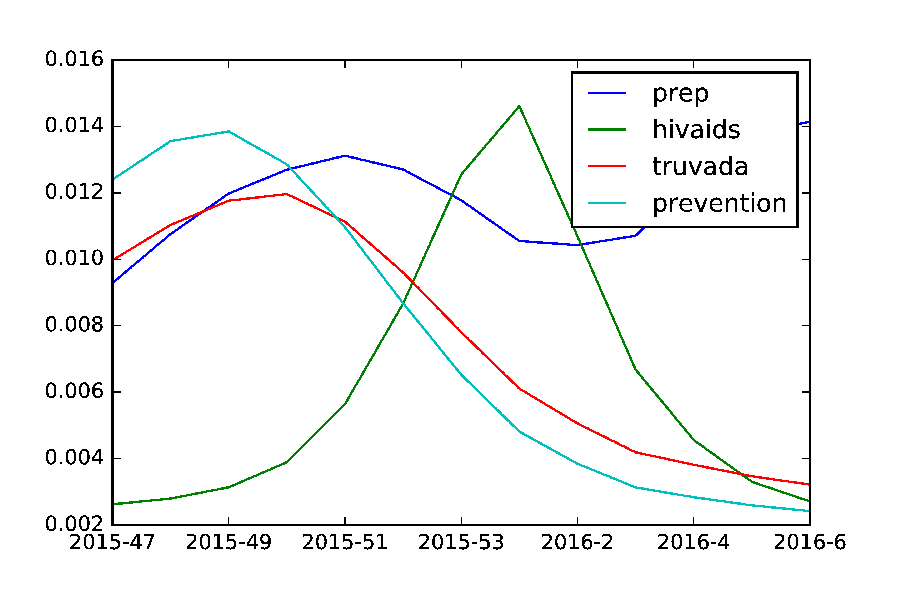
\includegraphics[height=2.5in, width=3.5in]{fig1}
\caption{DTM topic 3 word prevalence over time. Date is YYYY-WW.}
\end{figure}

% figure 3
\begin{figure}
\centering
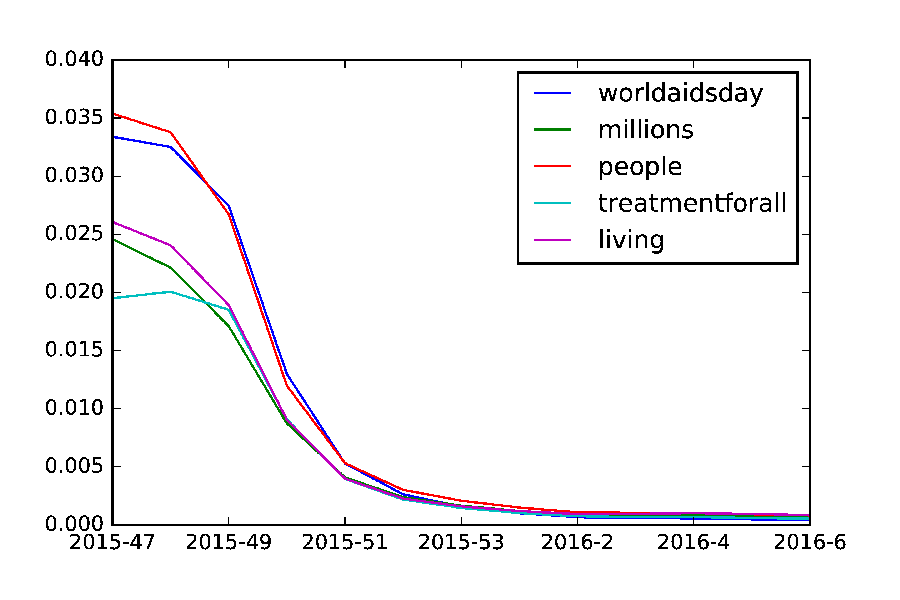
\includegraphics[height=2.5in, width=3.5in]{fig2}
\caption{DTM topic 5 word prevalence over time. Date is YYYY-WW.}
\end{figure}

\subsection{User Timeline Analysis}

Using a Paragraph2Vec analysis, we queried for the top 500 users related to '\#prep' who had at least 200 words in the combined set of tweets in their timeline, up to 3000 tweets. The timelines of these users were concatenated into 500 large timeline-documents. We then performed LDA on the timeline documents and identified words associated with 10 topics (Table 3). We can see some political, news and social media related keywords and colloquialisms in the top 5 words per topic.

A heatmap of Topics vs Users shows the distribution of topic assignment weighting over the 500 users (Figure 4). We can see that many of the users are mentioning things assigned to topics 2 and 8. Topic 2 appears to be related to certain geographic regions such as 'Nigeria' and 'Syria' that may be especially suffering from HIV. Topic 8 contains words such as 'giveaway' and 'startups' indicating that it may be related to social and economic coordination to combat HIV.

% table 3
\begin{table*}
\centering
\caption{Topics Present in 500 HIV/PrEP related Timelines}
\begin{tabular}{|l|c|c|c|c|c|} \hline
Topic ID & Word1 & Word2 & Word3 & Word4 & Word5\\ \hline
0 & 0.002*que & 0.001*por & 0.001*para & 0.001*milan & 0.001*een\\ \hline
1 & 0.001*yg & 0.001*ini & 0.001*yang & 0.000*aku & 0.000*breakingbad\\ \hline
2 & 0.001*lmao & 0.001*nigeria & 0.000*syria & 0.000*nigga & 0.000*kca\\ \hline
3 & 0.000*ntv & 0.000*inspiringthinkn & 0.000*ktnkenya & 0.000*haber & 0.000*tuscany\\ \hline
4 & 0.003*gurmeetramrahim & 0.001*ang & 0.001*ng & 0.001*ji & 0.001*ako\\ \hline
5 & 0.001*remedies & 0.000*tw & 0.000*mx & 0.000*rid & 0.000*momlife\\ \hline
6 & 0.000*flipboard & 0.000*mongolia & 0.000*gettingtozero & 0.000*blackburn & 0.000*occupy\\ \hline
7 & 0.002*newsbreakslive & 0.002*drudgereport & 0.000*woof & 0.000*und & 0.000*der\\ \hline
8 & 0.001*giveaway & 0.001*xx & 0.001*photography & 0.001*startups & 0.001*anc\\ \hline
9 & 0.001*realdonaldtrump & 0.001*lgbt & 0.001*hiring & 0.001*uniteblue & 0.001*tedcruz\\ \hline
\hline\end{tabular}
\end{table*}

\begin{figure}
\centering
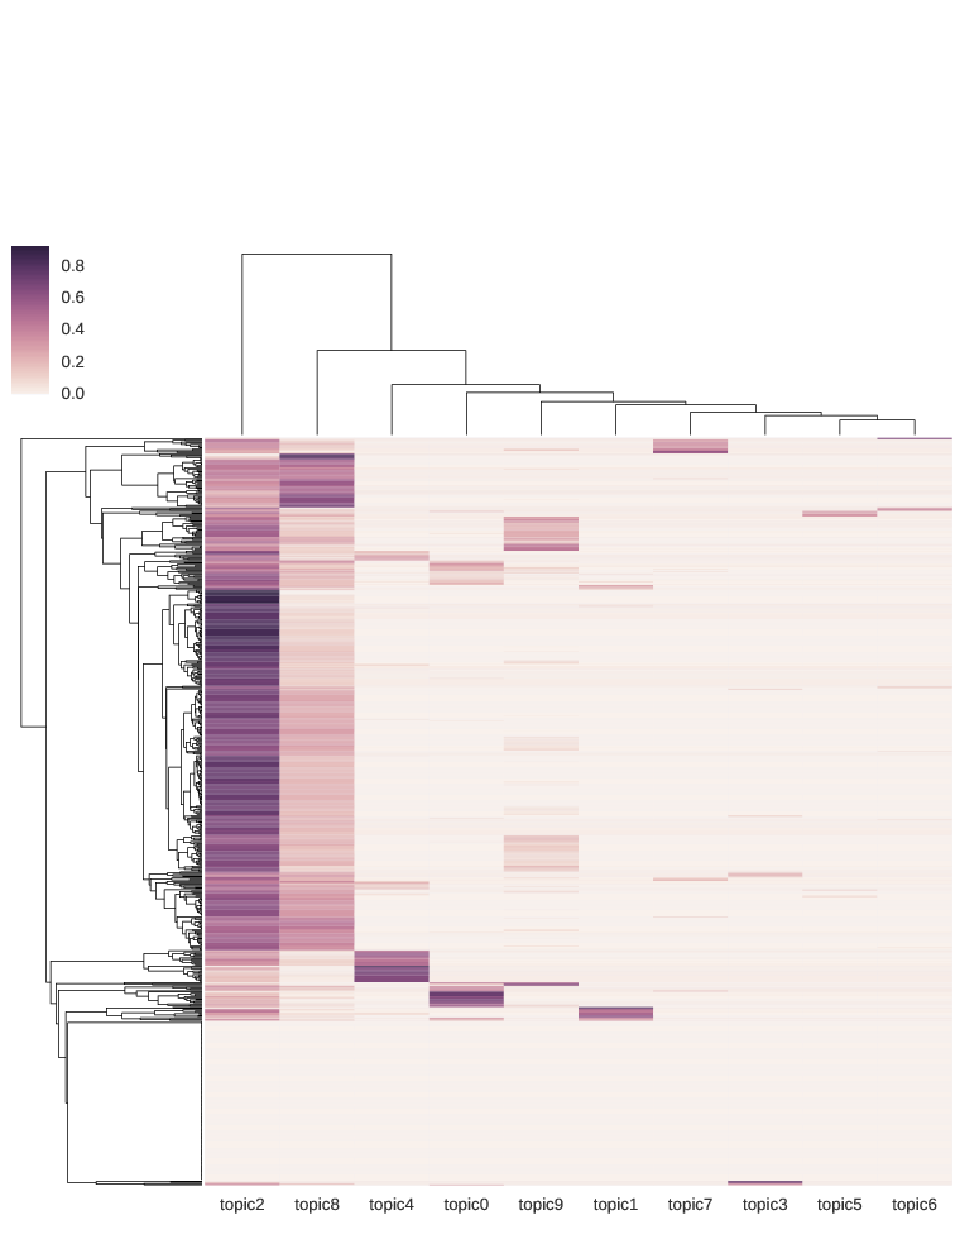
\includegraphics[height=2.5in, width=3.5in]{user_time}
\caption{Heatmap of Topics vs. Users.}
\end{figure}

\subsection{Sentiment Classification}

Lastly we sought to create a classification scheme to classify the sentiment of tweets either positive or negative. This classifier would allow us to quickly identify positive and negative PrEP related tweets to guide public health efforts. We first performed Paragraph2Vec on both our PrEP related tweet corpus and on another tweet corpus that had binary sentiment labels, positive, or negative. Then we trained a simple logistic regression classifier on the paragraph-vectors. We found that our classifier had an accuracy of 70\% on a validation set.

We then used this classifier to classify our PrEP related tweets into positive or negative labels. We reported the most positive, and most negative tweets, by log(probability), on our full dataset, and on tweets that specifically mention either 'prep' or 'truvada' (Table 4). It seems that overall the classifier seems to capture the sentiment relatively well, however it clearly fails to recognise the sarcasm present in the most positive overall tweet.

The sentiment results aren't perfect, but they do help us identify positive individials in PrEP and HIV public health such as user @greg0wen. The sentiment tweets also let us uncover some of the prevailing stigmas and negative sentiments surrounding PrEP usage.

\begin{table*}
\centering
\caption{Example Positive and Negative Sentiment Tweets}
\begin{tabular}{|l|p{10cm}|} \hline
Description & Tweet Body\\ \hline
Most Positive Overall & \#apple hey, apple, with your new headphone hack you are in the gouger camp of shkreli who hiked the hiv drug. nice going.\\ \hline
Most Positive PrEP & @greg0wen hi greg, I'm a hiv doctor and health writer doing a piece on hivprep could i poss contact you for some info? thanks, verity x\\ \hline
Most Positive Truvada & great skypeing the john grant just now about bowie , icelandic sagas and truvada! you're right elliot\_rose about the song disappointing!\\ \hline

Most Negative Overall & hiv sucks big time!! and I f\#n hate it!! We're almost there until this one stupid infection brought him back to where he started. sh\#t!!!\\ \hline
Most Negative PrEP & rt @SamNyembe can we attribute hivaids high rate in kzn to many men having not removed their prepuce? \\ \hline
Most Negative Truvada & this \#truvada convo has me catching feelings coz majority of men feel 0 responsibility for their reproductive \& sexual health\\ \hline

\hline\end{tabular}
\end{table*}


\section{Conclusions}

Conclusions go here.

Example citation (needed right now to compile):\cite{Lamport:LaTeX}

%\end{document}  % This is where a 'short' article might terminate

%ACKNOWLEDGMENTS are optional
\section{Acknowledgments}

Acknowledgements go here.

%
% The following two commands are all you need in the
% initial runs of your .tex file to
% produce the bibliography for the citations in your paper.
\bibliographystyle{abbrv}
\bibliography{sigproc}  % sigproc.bib is the name of the Bibliography in this case
% You must have a proper ".bib" file
%  and remember to run:
% latex bibtex latex latex
% to resolve all references
%
% ACM needs 'a single self-contained file'!
%
% no appendix for now...


\subsection{References}




\end{document}
